In this section we will detail the design of our tool, the algorithm and its parameters. 
\subsection{Algorithm}
\subsubsection{Input and output}
The algorithm accepts an X = n x k matrix of input data, and an Y = 1 x k  vector of expected data. It will evolve expressions that result, when evaluated on X, in an 1 x k vector Y' that approximates Y. N is the number of features, or parameters, the expression can use. K is the number of datapoints per feature. The algorithm makes no assumptions on the domain or range of the expressions or data set. While domain specific knowledge can be of great value, in real world situations such data is not always known.
\subsubsection{Control flow}
\begin{tikzpicture}[node distance=1.5cm, every node/.style={font=\footnotesize}]
\node (start) [startstop] {Start};
\node (phase) [decision, below of=start, yshift=-0.5cm] {Phase $<$ Phases};
\node (init) [process, below of=phase, yshift=-1cm] {0.0 Initialize};
\node (gen) [process, right of=init, xshift=4cm] {0.1 Generate random};
\node (while) [decision, below of=init, yshift=-1.5cm, align=center] {1. \\ Generation \\ $<$ \\ Generations }; % stopcondition?
\node (eval) [process, below of=while, yshift=-1.5cm] {2. Evaluate Population};
\node (select) [process, below of=eval] {3. Select};
\node (evolve) [process, below of=select] {4. Evolve};
\node (mutate) [process, right of=evolve, xshift=4cm, yshift = + 1 cm] {4.1 Mutate};
\node (crossover) [process, below of=mutate ] {4.2 Crossover};
\node (update) [process, below of=evolve] {5. Update Population};
\node (archive) [process, right of=while, xshift=4cm] {0.2 Archive};
\node (external) [process, right of=archive, xshift=4cm] {0.3 External};
\node (optimizea) [process, below of=archive] {6.1 Optimize};
\node (optimizet) [process, below of=update] {6.2 Optimize};

\draw [arrow] (start) -- (phase);
\draw [arrow] (phase) -- node[anchor=east]{yes}(init);
\draw [arrow] (init) -- (while);
\draw [arrow] (while) -- node[anchor=east]{yes}(eval);
\draw [arrow] (while) -- node[anchor=south]{no}(archive);
%\draw [arrow] (archive) -- (phase);
\draw [arrow] (eval) -- (select);
\draw [arrow] (select) -- (evolve);
\draw [arrow] (evolve) -- (mutate);
\draw [arrow] (mutate) -- (evolve);
\draw [arrow] (evolve) -- (crossover);
\draw [arrow] (crossover) -- (evolve);
\draw [arrow] (evolve) -- (update);
\draw [dashed, ->] (gen) -- node[anchor=south]{seeds}(init);
\draw [dashed, ->] (archive) -- node[anchor=south]{seeds}(init);
\draw [dashed, <->] (update) -- node[anchor=east]{optional}(optimizet);
\draw [dashed, <->] (archive) -- node[anchor=east]{optional}(optimizea);
\draw [dashed, <->] (external) -- node[anchor=south]{optional}(archive);
\draw [arrow] (archive)-- +(2,0) |- (phase) node[near start,sloped,above] {};

\draw [arrow] (update)-- +(-2,0) |- (while) node[near start,sloped,above] {};
\end{tikzpicture}
% High level overview
% UML

\subsubsection{Implementation}
Our tool is implemented in Python. The language offers portability, access to rich libraries and fast development cycles. The disadvantages are speed and memory usage compared with compiled languages (e.g. C++) or newer scripting languages (e.g Julia). % ref julia.
Furthermore, Python's usage of a global interpreter lock makes shared memory parallelism not feasible. Distributed programming is possible using MPI.

\subsection{Fitness}

\subsubsection{Distance function}
The goal of the algorithm is to find f' such that
\[Y = f(X)\]
\[Y' = f'(X)\]
\[dist(Y, Y') = e\]
e is minimal.\\
Not all distance functions are equally well suited for this purpose. A simple root mean squared error (RMSE) function has the issue of scale, the range of this function is [0, +$\infty$), which makes comparison problematic, especially if we want to combine it with other objective functions. A simple linear weighted sum requires that all terms use the same scale. 
Normalization of RMSE is an option, however there is no single recommended approach to obtain this NRMSE. \\
In this work we use a distance function based on the Pearson Correlation Coefficient. Specifically, we define 
\[
dist_p(Y, Y') = 1 - \vert r \vert
\]
with r
\[
r = \frac{\sum_{i=0}^{n}{(y_i-E[Y])*(y'_i-E[Y'])}}{\sqrt{\sum_{j=0}^{n}{(y_j-E[Y])^2}*\sum_{k=0}^{n}{(y'_k-E[Y'])^2}}}
\]
This function has a range [0,1] which facilitates comparison across domains and allows combining it with other objective functions.
The function reflects the aim of the algorithm. We not only want to assign a good (i.e. minimal) fitness value to a model that has a minimal distance, we also want to consider linearity between Y an Y'. 

\subsubsection{Diversity}\label{subsubdiversity}
Diversity, the concept of maintaining semantically different specimens, is an important aspect in metaheuristics. Concepts such as niching and partitioning are often used to promote this behavior, amongst other reasons to prevent premature convergence or even to promote multimodality.
Our tool uses a simple measure that mimics the more advanced techniques stated above. It should be clear that for any combination of input and output data, there are a huge set of expressions with an identical fitness value. Such expressions can lead to premature convergence, consider a population of 5 where the 3 best samples all have fitness scores of 0.134. Our tool will aim to prevent retaining expressions that have identical fitness values.
In contrast, in some metaheuristics \cite{DE} allowing replacement of solutions with identical fitness values (not duplication, but replacement), can actually help avoiding local minima. 

\subsubsection{Predictive behavior}
The algorithm evaluates specimens based on training data $X_t$, with $X_t$ a random sample from input data X of size j = r * k. R is the sampling ratio, the ratio between training and test data. K is the total amount of datapoints available per feature. 
After completion of the algorithm the population is ordered based on minimized fitness values calculated on the training data. 
In real world applications practitioners are also interested in the predictive qualities of the generates expression. In other words, how well do the expressions score on unknown data. In the final evaluation we score each expression on the full data to obtain this measure. 
While this gives us some information on how good an expression is on the full data set, what we would like to know is how the algorithm's progress is related to the value. For example, if we add 10 more generations, or increase the population by a factor 1.5, do we gain or lose in predictive quality of the expressions? To define this we use a correlation between the fitness values using the training data and those of the full data. 
This provides an immediate link between the two sets of values. 
Finally, we calculate a correlation trend between the training fitness values at the end of each phase, and the final fitness values calculated on the full data. This gives us good measure of how the algorithm will converge on a good solution on the full data. 

\subsubsection{Convergence limit}
As a stopcondition our tool uses a preset number of iterations. The user specifies the number of generations (g) and phases (r), and the algorithm will at most execute g x r iterations. Convergence stalling is implemented by keeping track of the number of successful operations (mutation or crossover). If this value crosses a threshold value convergence has stalled and the algorithm is terminated.


\subsection{Initialization}
Initialization is done using the 'full' method \cite{GP}. The algorithm has a parameter initial depth, each new expression in the population is created using that depth.
 
\subsubsection{Invalid expressions}\label{subsubinvalidexpressions}
Generating a random expression is done by generating random subtrees and merging them. A critical point to observe is that randomly generating expressions can be invalid for their domain. The ubiquitous example here is division by zero. Several approaches to solve this problem exist. One can define 'safe' variants of the functions, in case of division by zero, one can return a predefined value that will still result in a valid tree. The downside of this approach is that the division function's semantics is altered, a practitioner, given a resulting expression, would have to know that some functions are no longer corresponding entirely to their mathematical equivalents. 
The other option is assigning maximum fitness to an invalid expression. While simple, this approach needs a careful implementation. From a practical standpoint wrapping functions in exception handling code will quickly deteriorate performance. 
Our approach is quick domain check for each calculation, avoiding exceptions.

\paragraph{Invalidity probability}
We define the probability that a randomly generated tree of depth d, with n possible features, k possible base functions, and j data points as q. With more complex problems d will have to be increased. GP is also susceptible to bloat \cite{GPBloat}, increasing d even further. This issue will affect generation of subtrees in mutation. With more datapoints the probability of at least one leading to an invalid evaluation will increase linearly. An increase in d will lead to an exponential increase in the number of nodes in the tree. A node can be either a basefunction or a leaf (parameter or constant). For each additional node the probability q increases. We can conclude that q, while irrelevant for small problems and depths, becomes a major constraint for larger problem statements. 

\paragraph{Bottom up versus top down}
There are two methods to generate a tree based expression : bottom up and top down. The top down approach is conceptually simpler, we select a random node and add randomly selected child nodes until the depth constraint in satisfied. The problem with this approach is that the expression can only be evaluated at completion, early detection of an invalid subtree is impossible. 
In contrast a bottom up construction, where we generate small subtrees, evaluate them and if and only if valid merge them into a larger tree, allows for early detection of invalid expressions. A downside of this approach is the repeated evaluation of the subtrees. This can be mitigated by caching the result of the subtree.

\paragraph{Disallowing invalid expressions in initialization}
We can generate random expressions and let the evolution stage of the algorithm filter them out based on their fitness value, or we can enforce the constraint that no invalid expressions are introduced. The last option is computationally more expensive at first sight, since the algorithm is capable by definition of eliminating unfit expressions from the population. 
This can lead to unwanted behavior in the algorithm itself. For high q values we can have a significant part of the population that is at any one time invalid. This can lead to premature convergence, similar to a scenario where the population is artificially small or dominated by a set of highly fit individuals. Another observation to make is the algorithm will waste operations (mutation, crossover) on expressions that are improbable to contribute to a good solution. 
While more expensive computationally, we therefore prohibit generation of invalid expressions in the initialization. 

\subsection{Evaluation and cost}
Evaluating a tree requires a traversal, once for each datapoint. In order to compare optimization algorithms across implementations practitioners can use as a measure the number of evaluations required to reach a certain fitness level. If this measure is used, one should take into account that not all evaluations are equal. With the trees varying in depth and density the evaluation cost varies significantly. Furthermore, evaluation "1 + 2" is computationally far less expensive than "log(3, 4)".
Our tool uses a complexity measure that takes into account the density of the tree and which functions are used. A tree comprised of complex functions will score higher in cost than a corresponding tree using simple multiplications and additions. Although this is an option, we do not use this measure in the objective function. We would like to observe the effect of the cost, but not directly influence the algorithm. There is no direct link between more complex functions and an optimal solution. In certain domains the argument can be made that more complex functions are more likely to lead to overfitting, or more likely to lead to invalid trees (due to smaller domain).

\subsection{Evolution}
In the evolution stage we apply two operators on (a selection of) the population. The operators are configured to constrain the depth of the modified trees, enforcing the maximum depth parameter.
We trace the application of the operators during the execution using an effectiveness measure. Each time an operator application is able to lower the fitness of a tree, this measure increases. Using this measure we can gain insight when and how certain optimizations and modifications work inside the algorithm.

\subsubsection{Mutation}
Mutation works by selecting replacing a randomly chosen subexpression with a newly generated. In our implementation this means selecting a node in the tree and replacing it with a new subtree. Our mutation operator can be configured to replace the subtree with one of equal depth or a randomly chosen depth. The insertion point can be made depth-sensitive. A shallow node, a node with a low depth, is the root of a subtree with significant depth. Replacing such a subtree is therefore more likely to have a significant effect on the fitness value. Replacing a deep node will have on average a smaller effect. We will investigate this assumption in our experiments.
In our implementation the mutation operator is applied using a cooling schedule, or on the entire population. 
The cooling schedule uses the current fitness and the current generation of a tree to decide if mutation is likely to benefit from mutation. This is similar to the approach in simulated annealing. %ref
Mutation introduces new information into the optimization process (a new subtree). This process can be constructive (lowering fitness) or destructive (increasing fitness). The idea behind the cooling schedule is that for fitter trees the mutation operation will not be able to improve fitness (decrease it), while for less fit trees it has a higher probability. 
This probability is estimated using the current generation and fitness value (relative to the population), and using this information a random choice is made whether or not to apply mutation. In the experiments section we will investigate if this assumption holds, and if it leads to gains in fitness and or effectiveness.
The mutation operates has to generate new subtrees, and therefore the same issues seen in the initialization  process\ref{subsubinvalidexpressions} apply here as well. The mutation operator will use an invalid subtree, at the cost of having to generate subtrees until a valid one is found. If the depth sensitive operation proves to generate equal or better fitness values, this could significantly reduce the computation cost of the operator.

\subsubsection{Crossover}
Crossover operates on 2 trees in the population. It selects subtrees from both, and inserts them into each other. The resulting set of 4 trees is scored and the 2 fittest replace the original trees. As with mutation crossover can be configured to operate on a set depth, or pick a random depth. It can also work symmetric, picking an equal depth insertion point in both trees.
Crossover in our implementation can be applied in sequence to the entire population, with pairwise mating in order of fitness. Alternatively a random selection can be used. A variant of both, alternating between the two schedules based on a random choice is a third option. This last reflects in part the roulette wheel selection method, although without replacement. %ref
Crossover, unlike mutation, does not introduce new information in the sense that no new subtrees are generated. 
Crossover can be configured to work with a decreasing depth, operating only on deeper nodes at the later stages of the algorithm. The assumption for this mode of operation is similar to that made for mutation. 

\subsection{Selection}
After evolution a decision has to be made on which expressions will be retained in the population. In our tool the population is fixed, so a replacement is in order. We use an elitist approach. If a an expression has a lower (better) fitness value after mutation, it is replaced. 
In crossover we combine two expressions r, and t, resulting in two offspring s, u. 
From these four expressions the two with minimal fitness survive to the next generation.

\subsection{Archiving}
The algorithm holds an archive that functions as memory for best solutions obtained by seeding, from other processes, or the best expressions at the end of a phase.
At the end of a phase we store the j best expressions out of the population. J is a parameter ranging from 1 to the population size n. With j == n we risk premature convergence, with j == 1 the risks exists that we lose good expressions from phases which will have to be rediscovered. 
While there are numerous archiving strategies described in literature, we use a simple elitist approach. This means that there is no guarantee that the best j samples of phase i are retained, if they have fitness values lower than those present in the archive and the archive has no more empty slots, they will be ignored.
This leads us to the size of the archive. While no exact optimal value for this exists, in order to function as memory between phases it should be similar in size to the amount of phases. The j parameter will influence this choice as well.

\subsection{Representation and data structures}
\subsubsection{Expression}
We use a tree representation for an arithmetic expression, where each internal node represent a base function (unary or binary), and each leaf either a feature or a constant.

\paragraph{Tree representation}
We use a hybrid representation of a tree structure. The tree is a set of nodes, where each node holds a list of children nodes. This representation favors recursive traversal algorithms. In addition to this representation, the nodes of tree are stored in a dictionary keyed on the position of a node. This allows for O(1) access needed by the mutation and crossover operators. The overhead of this extra representation is minimal, since the keys are integers and only a reference is stored. A list representation would be faster in (indexed) access, but would waste memory for sparse trees. With a mix of unary and binary operators the average nodecount of a tree with depth d is $\frac{2^{d+1}-1  + d}{2}$ = O($2^d$) resulting in savings on the order of $2^d$, with d the depth of the tree.
The algorithm has the choice which mode of access to use depending on the usage pattern. As an example, selecting a random node in the tree is O(1), selecting a node with a given depth is equally O(1). Splicing subtrees is equally an O(1) operation.

\paragraph{Base functions}
The set of base functions is determined by the problem domain. For symbolic regression we use the following set:\\
+, -, \%, /, max, min, abs, tanh, sin, cos, tan, log, exp, power\\
A problem with this set is the varying domain of each, why may or may not correspond with the domain of the features. A possible extension is to use orthogonal base functions such as Chebyshev polynomials. In our solution the functions listed correspond with their mathematical equivalent, e.g. division by zero is undefined. Other constraints are based on floating point representation (e.g overflow).

\paragraph{Constants}
Constants are fixed values in leaves in the tree. The representation also allows for multiplicative weights for each node, which can be used to optimize the final solution. In contrast to the base functions with a limited set to choose from, constants have the entire floating point range at their disposal. The probability of selecting a 'right' value is nearly non existent, and domain information is lacking for these constants, it depends on the entire subtree holding the constant. We select a constant from a small range and allow the algorithm to recombine these constants later to larger values. This limiting of the search space can lead to the algorithm converging faster to a suboptimal solution.
% TODO reference main explanation of const optimization problem
The constants are reference objects in the tree, and so can be accessed and modified in place by an optimizer.

\paragraph{Features}
Features are represented as an object holding a reference to a set of input values, and always occur as leaves. The choice for a random leaf is evenly distributed between constants and features.

\subsubsection{Population}
The population of trees is kept in a sorted dictionary, where the key is the fitness value and the value is a reference to the tree representing the expression. 
This representation allows for fast access in selecting a (sub)set of fittest trees. It also allows for an O(1) check if we already have an equivalent solution, a tree with a fitness score which we already have in the population. This allows our diversity approach mentioned in \ref{subsubdiversity}.

\subsection{Parameters}
In this section we briefly list the main parameters of the algorithm and their effects on convergence, runtime and complexity.
\subsubsection{Depth}
The depth of trees van vary between an initial and maximum value. If we know in advance an optimal solution uses 13 features, the tree should have at least 13 leaves in order to use each feature once. This requires a depth of at least 4. In practice the depth will need to be greater due to the use of unary functions, and bloat. Bloat is a known issue in GP %ref
where the algorithm, unless constrained by limits or an objective function that penalizes depth, will tend to evolve deep trees without gaining much in fitness.
A similar problem arises with the generation of constants. Suppose we would like to generate the constant 3.14, the probability of generating this by a single random call is extremely small. The algorithm will try to build an expression fitting 3.14. The problem with this is that this process is highly inefficient and uses nodes that could otherwise be used to approximate the expected values. 
Without a solution for this issue, the user would have to take this into account and increase the depth parameter. 
From \ref{subsubinvalidexpressions} we know that the initialization process and the mutation operator will become more costly exponentially with the increase in depth.
A similar argument can be made for the time and space complexity of operating on deeper trees, both increase exponentially.

% complexity
\subsubsection{Populationsize}
The population size is directly related to convergence speed. The catch is the quality of the solution, a very small population will lead to premature convergence, the population is lacking in diversity (or information viewed from a different perspective).
A large population on the other leads to a large increase in runtime, unless the operators only work on a subset of the population. The optimal value is problem specific, but values in the range of 20-50 gives (for this tool) a good balance.

\subsubsection{Phases and generations}
The execution of the algorithms comprises of g generations and r phases, resulting in a maximum of g x r iterations. 
For both parameters a too small value will hinder convergence, while a high value can lead to overfitting. The optimal value is domain specific and dependent on the iterations required to approximate the expected data. This is by virtue of the problem statement unknown. There is a subtle difference in both. Each phase a reseed of the algorithm is done using the archive. This archive holds the best results from previous phases, external seeds and in a distributed setting the best best solutions from other processes.
The remainder of the population is initialized with random tree. These trees introduce new information into the optimization process, and while expensive and with a low probability of improving fitness, nonetheless will help avoid premature convergence. 
If the archive size is less than the population size, new trees will always be introduced. The rate at which the archive fills is dependent on the number of phases and a parameter which determines how many trees are archived. In a distributed setting this process accelerates using the input of other processes. If the archive is full after i phases, and the archive size is equal to the population, further phases will no longer have the benefit of newly generated trees. This does not prevent convergence, but could reduce the convergence rate in some scenarios.

\subsubsection{Samples}
The user can provide the algorithm with input data, or can specify a range from which to sample the input data. In addition, the ratio between training and testing data can be adjusted. Care should be taken in tuning this value. A low ratio will increase the probability that evolved solutions are invalid on the test data, while a high ratio will lead to overfitting.

\subsubsection{Domain}
Knowing the domain of the problem can significantly reduce the time needed to converge to a solution. In our implementation we assume no domain knowledge. While this increases the complexity of obtaining a good solution, it also makes for a more fair evaluation of the algorithm and optimizations used. 

\subsection{Incremental support}
Our tool support incremental operation. The user can provide seeds, expressions that are known or assumed to be good initial approximations. The algorithm writes out the best solutions obtained in an identical format. By combining this the user can create a Design Of Experiment (DOE) setup using the algorithm. As a use case, suppose the user wants to apply symbolic regression on the output of an expensive simulation. The simulator has k features or parameters, each with a different domain and j datapoints. The user wants insights into the correlation of the parameters. 
A naive approach would be to generate output data for a full factorial experiment, and feed this into the CSRM tool. For both the simulator and the SR tool the cost of this approach would be prohibitive. It is likely that some features are even irrelevant, leading to unnecessary computation. Instead we can opt for a combined DOE approach. We start with a subset of features k' $<$ k and datapoints j' $<$ k. The simulation results Q of this subset are then given to the CSRM algorithm. It generates a solution, optimized for this subset of the problem. 
The user then adds more parameters, k' $<$ k'' $<$ k and/or datapoints j' $<$ j'' $<$ j, runs the simulator again. The resulting output is given the CSRM tool, with Q as seed. This seed is used as memory of the previous run on the smaller input set. Unless there is no correlation between the incrementing datasets the CSRM tool can use the knowledge gained from the previous run to obtain faster convergence for this new dataset. In addition, by inspecting Q the user can already analyze a (partial) result regarding the initial parameter set. Suppose k = 5, and only 3 parameters are used in Q. Then the user can exclude the missing two parameters from the remainder of the experiment, as these are unlikely to contribute to the output.
By chaining the simulator and CSRM tool together in such a way, an efficient DOE approach can potentially save both simulation and regression time, or result in increased quality of solutions. 
The advantages are clear :
\begin{itemize}
\item The SR tool can start in parallel with the simulator, instead of having to wait until the simulator has completed all configurations.
\item Reducing irrelevant parameters detected by the SR tool can save in configuration size for the simulator.
\item The SR tool can reuse previous results as seeds, and tackles and slowly increasing search space with those initial values instead of starting without knowledge in a far larger search space.
\end{itemize}
Possible disadvantages are :
\begin{itemize}
\item The SR tool is not guaranteed to return the optimal solution, it is possible the process is misguided by suboptimal solutions. This risk exist as well in the full approach.
\item Interpretation of the results can be needed in order to make the decision to prune features.
\end{itemize}
We will investigate this approach in our use case in  \ref{secexperiments}.
The following diagram illustrates a DOE hypercube design using our tool and a simulator. \\
\begin{tikzpicture}[node distance=1.5cm, every node/.style={font=\footnotesize}]
\node (start) [startstop] {Start};
\node (featureset) [process, below of=start] {Features};
\node (datapoints) [process, below of=featureset] {Datapoints};
\node (x) [process, right of= datapoints,xshift=4cm, yshift=1cm] {X};
\node (simulator) [process, right of=x, xshift=4cm] {Simulator};
\node (srtool) [process, below of=x] {SR Tool};
\node (expressions) [process, below of=srtool] {Expressions};
\node (analyze) [process, below of=datapoints] {Analyze};

\draw [arrow] (featureset) -- +(+2,0) |-(x) node[near start,sloped,above]{};
\draw [arrow] (start) --(featureset);
\draw [arrow] (datapoints) -- +(+2,0) |-(x) node[near start,sloped,above]{};
\draw [arrow] (x) --node[anchor=south]{input}(simulator);
\draw [arrow] (x) --(srtool);
\draw [arrow] (simulator) -- (srtool)node[anchor=south]{Y};
\draw [arrow] (srtool) --node[anchor=east]{generates}(expressions);
\draw [arrow] (expressions)-- +(+2,0) |- (srtool) node[near start,sloped,below, anchor=south] {seeds};
\draw [arrow] (expressions)-- +(-2, 0) |- (analyze) node[near start,sloped,above, anchor=south] {};
\draw [arrow] (expressions)-- +(-2, 0) |- (analyze) node[near start,sloped,above, anchor=south] {};
\draw [arrow] (analyze)-- +(-2, 0) |- (featureset) node[near start,sloped,above, anchor=south] {};
\draw [arrow] (analyze)-- +(-2, 0) |- (datapoints) node[near start,sloped,above, anchor=south] {reduces/expands};
\end{tikzpicture}

\subsection{Statistics and visualization}
Stochastic algorithms are notoriously hard to debug. By virtue of the problem statement we do not know whether the rendered solution is what is expected. The size of the search space makes detecting edge cases impossible. In addition the algorithm functions as a black box, where output is presented to the user without a clear trace indicating how or why this output was obtained. Both for developer and practitioner insight into the algorithms inner workings is vital. 
Our tool provides a wealth of runtime statistics ranging from fitness values per expression for each point in the execution, convergence behavior over time, depth and complexity of the expressions, cost of evaluations, effectiveness of operators, correlation between training en test fitness values and more. These statistics can be saved to disk for later analysis, or displayed in plots in a browser. Using this information the user can tune the parameters of the algorithm (e.g. overfitting due to an excessively large number of phases), the developer can look at how effective new modifications are (e.g. new mutation operator) and so on.
It is even possible to trace the entire run of the algorithm step by step by saving the expressions in tree form, displayed in an SVG image rendered by Graphviz \cite{graphviz}. In Figure \ref{fig:viz} a selection of the collected statistics on a testfunction is shown. The third testproblem was used with a depth in [4,10], 30 generations, populationsize 30, and 4 phases.
% Add examples of visualization here
 \begin{figure}
    \centering
    \begin{subfigure}{0.5\textwidth}
    \centering
        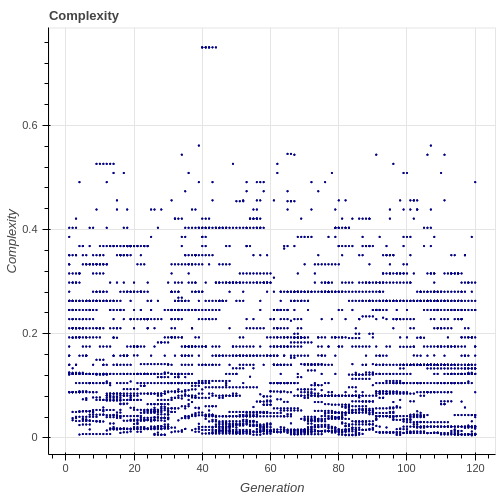
\includegraphics[width=0.8\linewidth]{figures/viz_complexity.png}
        \caption{Scaled complexity over generations.}
    \end{subfigure}%
    \begin{subfigure}{0.5\textwidth}
    \centering
        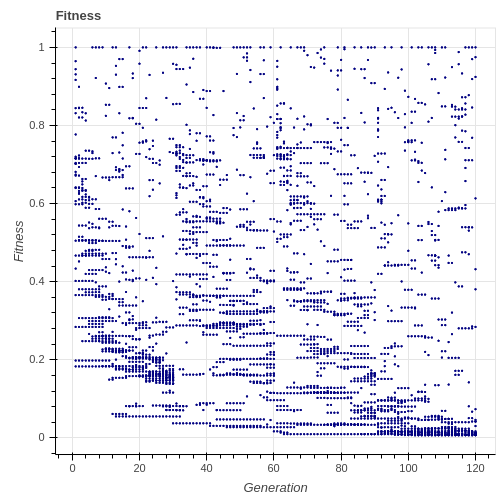
\includegraphics[width=0.8\linewidth]{figures/viz_fitness.png}
        \caption{Fitness values over generations.}
    \end{subfigure}
        \begin{subfigure}{0.5\textwidth}
    \centering
        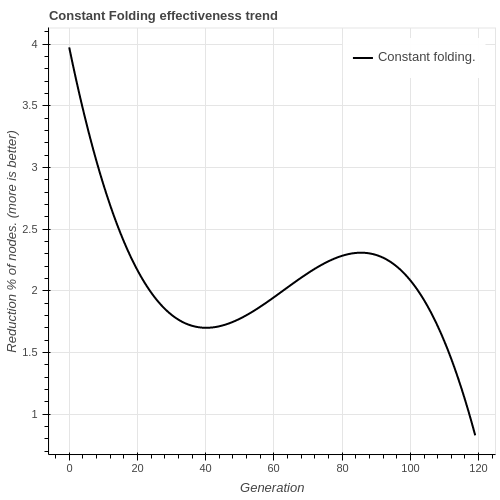
\includegraphics[width=0.8\linewidth]{figures/viz_constantfoldingtrend.png}
        \caption{Constant folding savings.}
    \end{subfigure}%
    \begin{subfigure}{0.5\textwidth}
    \centering
        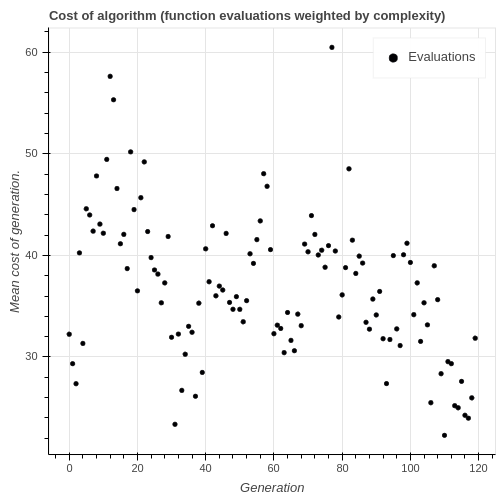
\includegraphics[width=0.8\linewidth]{figures/viz_meancost.png}
        \caption{Mean evaluation cost.}
    \end{subfigure}
        \begin{subfigure}{0.5\textwidth}
    \centering
        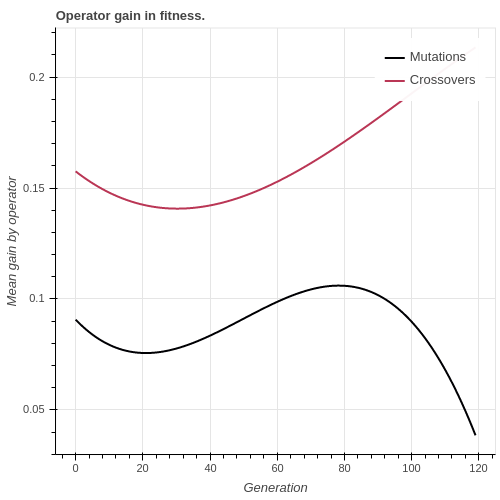
\includegraphics[width=0.8\linewidth]{figures/viz_operatorgaintrend.png}
        \caption{Operator gain.}
    \end{subfigure}%
    \begin{subfigure}{0.5\textwidth}
    \centering
        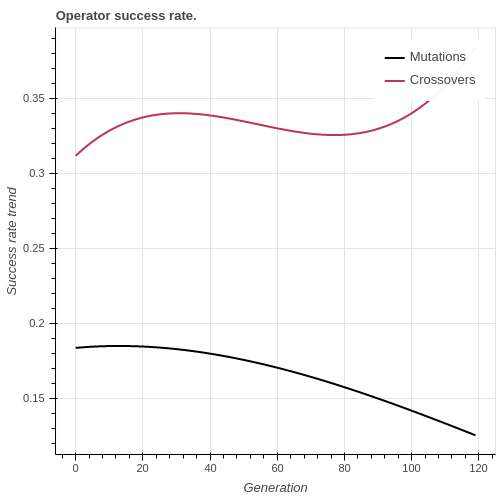
\includegraphics[width=0.8\linewidth]{figures/viz_operatorsuccessratetrend.png}
        \caption{Operator success rate.}
    \end{subfigure}
    \caption{Selection of visualizations generated by CSRM.}
    \label{fig:viz}
    \end{figure}

\subsection{Conclusion}
In this section we have covered in detail the design of the CSRM tool, highlighting the choices made. 
% Full featured tool offers insight, variation, testing.
% 
